\documentclass[a4paper]{report}

% \usepackage[utf8]{inputenc}
% \usepackage[T1]{fontenc}
% \usepackage{textcomp}
\usepackage[english]{babel}
\usepackage{amsmath, amssymb}
\usepackage[separate-uncertainty=true, multi-part-units=single]{siunitx}
\usepackage[]{subfig}
\usepackage[colorlinks=true, anchorcolor=blue, linkcolor=blue, citecolor=blue, bookmarks=false,hyperfootnotes=false]{hyperref}
\usepackage[margin=1in]{geometry}
\usepackage{color,soul}
\usepackage{tabularx}

% figure support
\usepackage{import}
\usepackage{xifthen}
\pdfminorversion=7
\usepackage{pdfpages}
\usepackage{transparent}
\usepackage{physics}
\graphicspath{ {./figures/} }
% \setlength{\parindent}{0pt}
\usepackage{chngcntr}
\usepackage{verbatim}
\usepackage{indentfirst}
\usepackage[most]{tcolorbox}
\numberwithin{equation}{section}
\counterwithin{figure}{section}
\newcommand{\incfig}[1]{%
		\def\svgwidth{\columnwidth}
		\import{./figures/}{#1.pdf_tex}

}

\pdfsuppresswarningpagegroup=1

% for citations / references
\usepackage[style=ieee]{biblatex}
\addbibresource{styx-report.bib}

\begin{document}

%----------------------------------------------------------------------------------------
%	TITLE PAGE
%----------------------------------------------------------------------------------------
\begin{titlepage} % Suppresses displaying the page number on the title page and the subsequent page counts as page 1
	\newcommand{\HRule}{\rule{\linewidth}{0.5mm}} % Defines a new command for horizontal lines, change thickness here
	
	\center % Centre everything on the page
	%------------------------------------------------
	%	Headings
	%------------------------------------------------
	
	\textsc{\LARGE Rheinische Friedrich-Wilhelms-Universit\"at Bonn }\\[4cm] % Main heading such as the name of your university/college
	
	\textsc{\Large Advanced Laboratory Course}\\[0.5cm] % Major heading such as course name
	
	\textsc{\large Performed on: May 12 - 13, 2022}\\[0.5cm] % Minor heading such as course title

	\textsc{\large Submitted on: June 20, 2022}\\[0.5cm] % Minor heading such as course title
	
	%------------------------------------------------
	%	Title
	%------------------------------------------------
	
	\HRule\\[0.4cm]
	
	{\huge\bfseries E217: STYX}\\[0.4cm] % Title of your document
	
	\HRule\\[1.5cm]
	
	%------------------------------------------------
	%	Author(s)
	%------------------------------------------------
	
	\begin{minipage}{0.4\textwidth}
		\begin{flushleft}
			\large
			\textit{Authors}\\
			Keito Watanabe \\
			Paarth Thakkar
		\end{flushleft}
	\end{minipage}
	~
	\begin{minipage}{0.4\textwidth}
		\begin{flushright}
			\large
			\textit{Tutor(s)}\\
			Patrick Bauer
		\end{flushright}
	\end{minipage}

	\vspace*{5em}

	\begin{minipage}{0.8\textwidth}
		\begin{centering}
			% \large
			\textbf{Abstract}\\[0.2cm]
            
		\end{centering}
	\end{minipage}
	
	% If you don't want a supervisor, uncomment the two lines below and comment the code above
	%{\large\textit{Author}}\\
	%John \textsc{Smith} % Your name
	
	%------------------------------------------------
	%	Date
	%------------------------------------------------
	
	%\vfill\vfill\vfill % Position the date 3/4 down the remaining page
	% \vfill\vfill
	
	% {\large\today} % Date, change the \today to a set date if you want to be precise
	
	%------------------------------------------------
	%	Logo
	%------------------------------------------------
	
	%\vfill\vfill
	%\includegraphics[width=0.2\textwidth]{placeholder.jpg}\\[1cm] % Include a department/university logo - this will require the graphicx package
	 
	%----------------------------------------------------------------------------------------
	
	% \vfill % Push the date up 1/4 of the remaining page
	
\end{titlepage}



\tableofcontents

\chapter{Introduction} \label{chap:intro}

...

In this report, we closely follow \cite{labman}.

\chapter{Theory} \label{chap:theory}

\section{Cosmic Rays}



Primary cosmic rays are highly energetic charged particles or nuclei with a long lifetime of order $10^6$ years or longer that are accelerated by 
astrophysical origins. These particles mainly consist of protons (85\%), but also consist of heavier nuclei such as Helium \cite{Tanabashi2018}. 
These cosmic rays propagate through intergalactic and interstellar space, losing energy through radiative processes \cite{DeDomenico2012}.
They are then captured by the Earth's magnetic field before arriving at Earth's atmosphere with energies in MeV to GeV ranges. 
They then interact with the atmospheric nuclei on Earth, producing "secondaries", that is, particles produced from such interactions. The secondaries
produced are mainly pions ($\pi^\pm, \pi^0$), whereas kaons ($K^\pm, K^0, \bar{K}^0$) are only produced with a probability of 10\% compared to pions \cite{Grupen2005}. \par 

\begin{figure*}[!h]
	\centering
	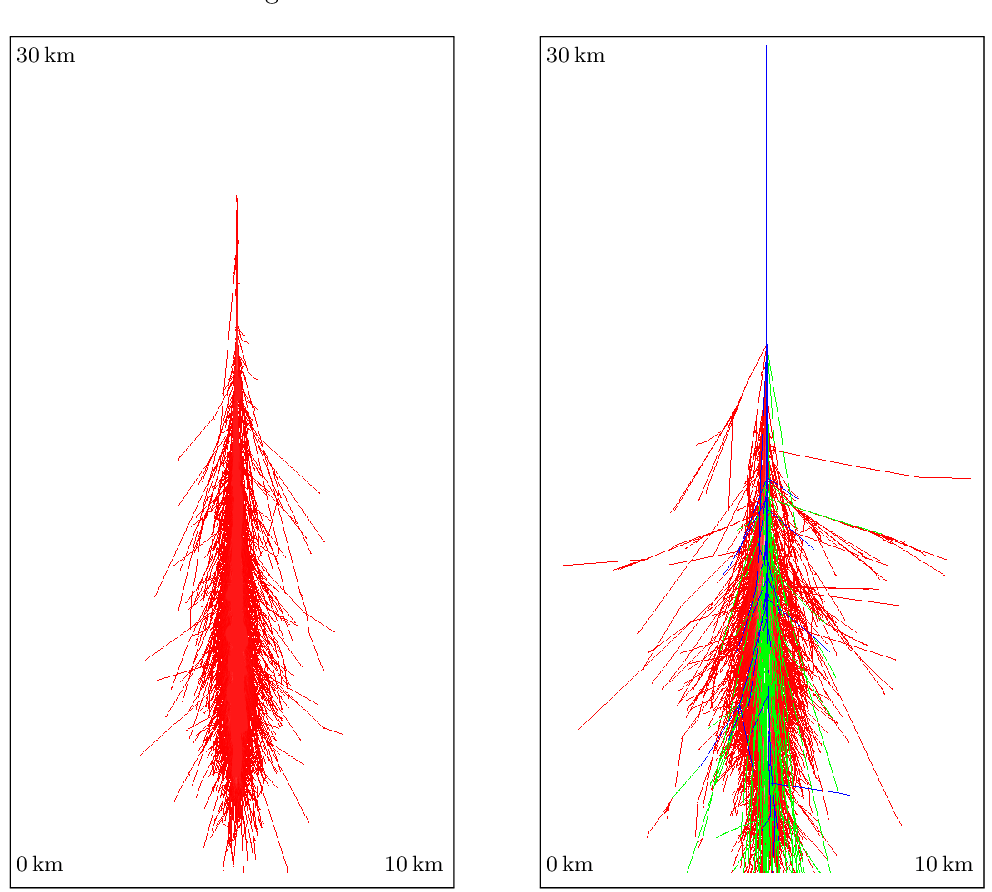
\includegraphics[width=0.6\textwidth]{em_hadronic_showers.png}
	\caption{ \textit{Left:} An electromagnetic shower induced by $\gamma$ at $\SI{1}{\tera\electronvolt}$. 
				\textit{Right: } A hadronic shower induced by a $\SI{1}{\tera\electronvolt}$ proton. Both plots show the lateral
				development of the showers at different altitudes. The red lines indicate electromagnetic components, blue indicates 
				hadronic components, and green indicate muon components (consisting of $\mu, \nu_\mu$). Obtained from Ref. \cite{Haeffner2014}. }
	\label{fig:em_had_showers}
\end{figure*}

As pions and kaons are not stable, they decay into subsequent particles through various channels.  
The neutral pion most commonly decay into a pair of photons ($\pi^0 \rightarrow \gamma + \gamma$), which subsequently produces a pair of electron and positron (pair production). They then undergo 
subsequent annihilation and bremsstrahlung processes, creating an electromagnetic cascade consisting of these three particles. Charged 
pions and kaons, however, primarily decay into a pair of muon and its corresponding neutrino or anti-neutrino ($\pi^+, K^+ \rightarrow \mu^+ + \nu_\mu$, $\pi^-, 
K^- \rightarrow \mu^- + \bar{\nu}_\mu$). These muons can also decay weakly into electrons, which then create subsequent electromagnetic cascades.
At higher energies of $E > \SI{10}{\giga\electronvolt}$, these pions and kaons can also decay into subsequent pions, which 
creates a hadronic cascade primarily consisting of these particles. Fig. \ref{fig:em_had_showers} shows an example of an electromagnetic and hadronic cascade that occurs from cosmic rays.


Through such electromagnetic and hadronic cascades, most charged particles are absorbed by the atmosphere and thus do not reach sea level. However, most of the muons 
produced from pions and kaons reach sea level due to their long lifetime, and as such approximately 80\% of the charged particles that reach sea level are muons.
The flux of muons detected at sea level is approximately 1 particle per cm$^2$ per minute, and as such one can detect more than $7 \times 10^{6}$ muons for an 
overnight measurement with a detector with an area of $\SI{1}{\meter\squared}$.  Neutrinos also reach sea level as they only interact weakly with matter and has a 
low interaction probability \cite{Grupen2005}. In the setup of our experiment, however, we are not able to detect neutrinos and thus only muons are detected. 
Fig. \ref{fig:air_shower} shows the schematic of a typical air shower from a primary cosmic ray. \par 


\begin{figure*}[!h]
	\centering
	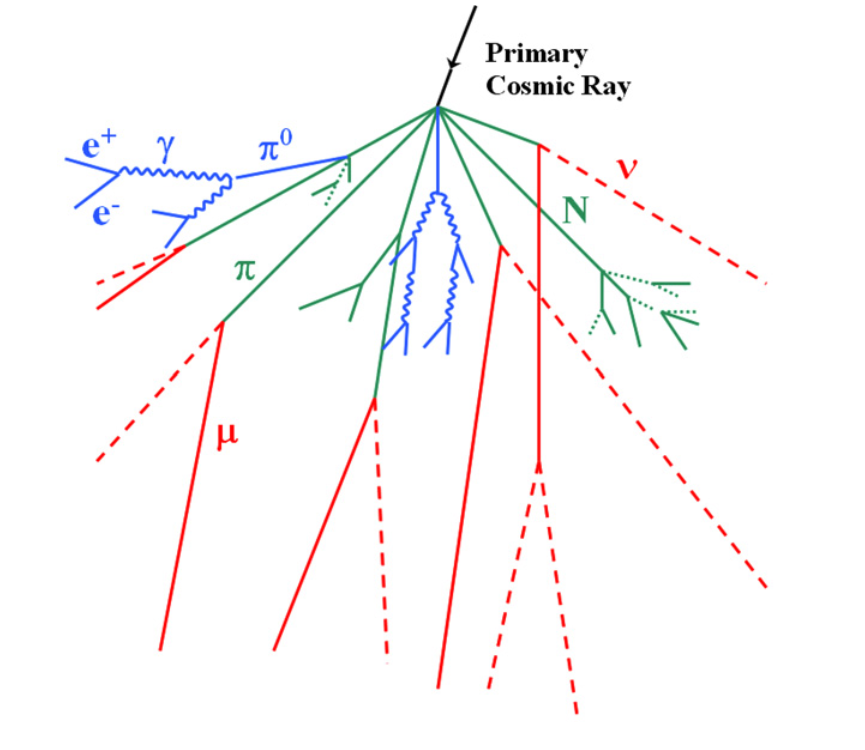
\includegraphics[width=0.6\textwidth]{air_shower.png}
	\caption{A typical air shower resulting from interaction of primary cosmic ray with the atmosphere. Electromagnetic cascades are shown in blue and hadronic 
	cascades are shown in green. The muons and neutrinos (indicated in red) produced from pion and kaon decays are the most common particles that reach sea level.
	Obtained from Ref. \cite{Blanco2009}.}
	\label{fig:air_shower}	
\end{figure*}

The total muon intensity distribution depends on the zenith angle $\theta$, i.e. the angle from the local zenith of the location of 
measurement. Such dependence is due to the stronger absorption of muons as they have to propagate through larger distances at 
inclined angles. The intensity distribution is given as such: 
\begin{equation}
    I(\theta) = I_0 \cos^n \theta 
\end{equation}
where $I_0$ is the intensity at the local zenith ($\theta = 0^\circ$) \cite{Grupen2005}. The exponent of the cosine function at 
sea level is $n = 2$ as most muons have energies $E_\mu \sim \SI{3}{\giga\electronvolt}$ when they reach sea level \cite{Stefano2012}.

\section{Gaseous Detectors}

To detect the muons that originate from cosmic ray showers, we use ionization detectors which collects the ionized electrons and ions 
from the emitted radiation from such muons. The basic configuration of an gaseous ionization detector is 
made of a cylindrical container with conducting walls, representing the cathode, that is filled with a noble gas such as argon. A positive voltage 
$+V_0$ is applied through a conducting wire, representing the anode, which is then connected to the thin end window.
See Fig. \ref{fig:ionization_chamber_schematic} 
for a schematic of the ionization detector with this setup. From this, a radial electric field of the following form is generated within the chamber:
\begin{equation}
	E(r) = \frac{1}{r}\frac{V_0}{\ln (b / a)}
\end{equation}
where $r$ is the radial distance from the axis, $b$ is the inner radius of the cylinder, and $a$ is the outer radius of the conducting 
wire as shown in Fig. \ref{fig:ionization_chamber_schematic}. \par 

\begin{figure*}[!h]
	\centering
	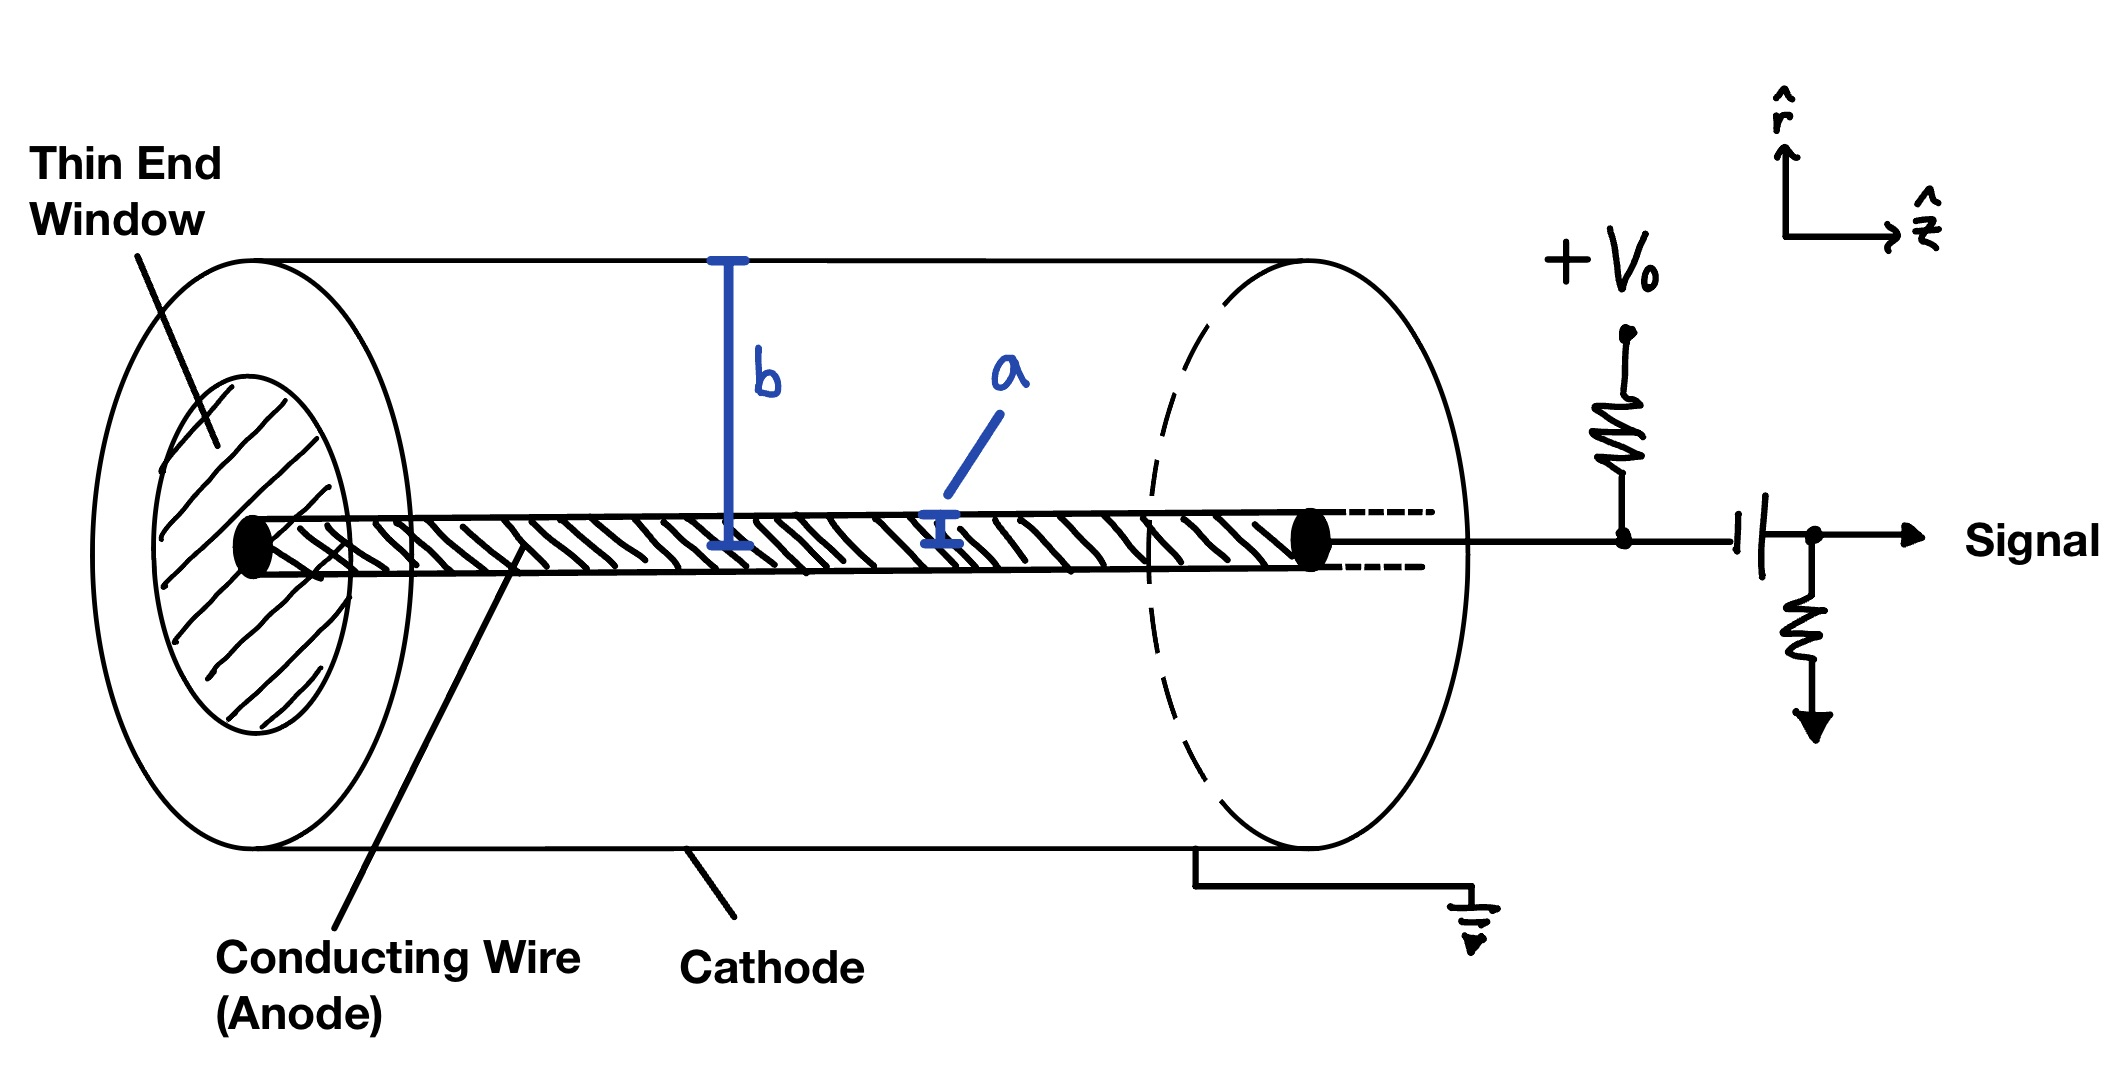
\includegraphics[width=0.6\textwidth]{ionization_chamber_schematic.png}
	\caption{Schematic of an gaseous ionization detector based on Ref. \cite{Leo1994}. Here, $b$ is the inner radius of the cylinder (cathode) and $a$ is the outer radius 
	of the conducting wire (anode).}
	\label{fig:ionization_chamber_schematic}	
\end{figure*}

As such, as the charged particles traverses through the detector it produces electron-ion pairs. Due to the resulting electric field, 
the electrons and ions drift towards the anode and cathode respectively. The signal from the anode can then be used for detection of the 
traversing charged particle \cite{Leo1994}. \par 

The signal obtained from the ionization detector depends on the field intensity and thus the applied voltage $V_0$. Fig. \ref{fig:ionization_regions} shows the 
dependency of the number of ions collected with the applied voltage for two types of incident particles. This dependence can be separated into six regions:
\begin{enumerate}
	\item \textbf{Recombination Region}: For low voltages, the electric field is not strong enough to accelerate the electron-ion pairs, thus allowing them to recombine 
			before they are collected.
	\item \textbf{Ionization Region}: At some voltage, enough voltage is applied so that all electron and ions are collected in their respective electrodes. 
			A plateau is observed in this region as increasing the voltage will not affect the number of ions or electrons collected. Ionization chambers operate in this region.
	\item \textbf{Region of Proportionality}: If we increase the voltage past the plateau region, the electric field is strong enough to accelerate the electrons to ionize the gas molecules 
			in the cylinder. Electrons produced from the ionization will further ionize other gas molecules, creating an ionization avalanche or cascade. As $E \propto r^{-1}$,
			the electric field is strongest near the anode so the avalanche occurs very quickly before electrons are collected by the anode. Since the number of electron-ion
			pairs are directly proportional to the number of primary electrons, the number of ions collected is proportional to the applied voltage $V_0$. Proportionality
			chambers are operated within this region, and is the most relevant region for our experiment.
	\item \textbf{Region of Limited Proportionality}: As we increase the voltage further, the proportionality is lost as the space charges distorts the electric field
			near the anode. 
	\item \textbf{Saturation Region}: Further increasing the voltage, the increased energy causes discharge within the gas. A chain reaction of avalanches occur 
			throughout the anode, causing the output signal to be saturated. The amplitude of the signal will remain the same even when increasing the energy, 
			yielding the second plateau. To prevent this effect, a quenching gas is often placed in the medium to absorb the photons causing the chain reaction. 
			Geiger-M{\"u}ller counters operate in this region.
	\item \textbf{Discharge Region}: Above the saturation region, continous discharge occurs throughout the cylinder which can damage the detector. As such, this region
			is to be avoided when operating the detector.
\end{enumerate}

\begin{figure*}[!h]
	\centering
	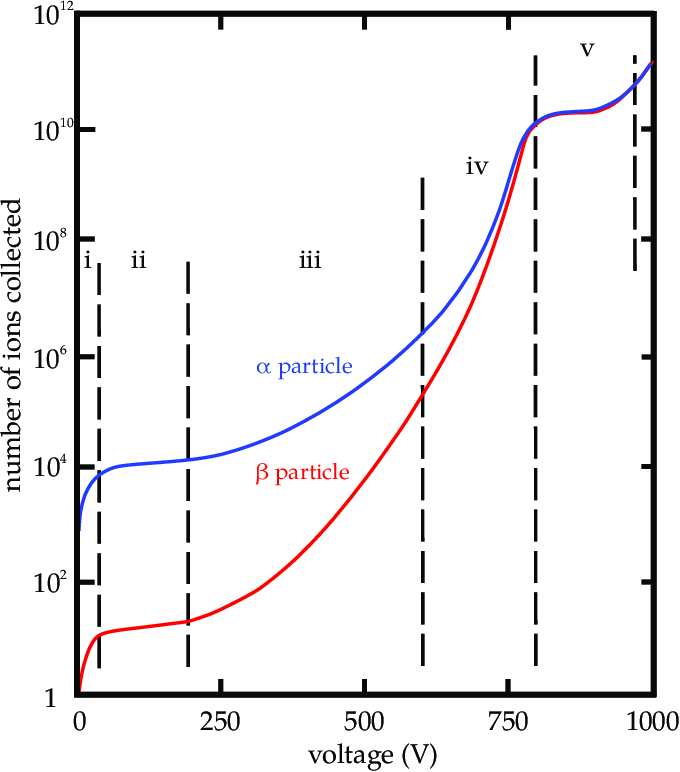
\includegraphics[width=0.5\textwidth]{ionization_regions.png}
	\caption{Number of ions collected at different applied voltage where the incident particles are $\alpha$ or $\beta$ particles. 
	The first five regions as mentioned in the script are labelled (i) - (v) in the plot, and the sixth region can be seen to the right of region (v). 
	Obtained from Ref. \cite{Lukas2018}. }
	\label{fig:ionization_regions}	
\end{figure*}

\section{Drift Chambers}

In our experiment, we use a type of proportional chamber called a drift chamber, also known as "straws". The drift chamber allows one to determine the spatial information 
of the traversing particle by measuring the drift time of the ionized electrons. The position of the produced electrons from the anode wire is 
given as such: 
\begin{equation}
	x = \int_{t_0}^{t_1} u dt
\end{equation}
where $t_0$ is the arrival time of the particle, $t_1$ is the time in which the signal reaches the anode, and $u$ is the drift velocity. To obtain a 
linear depedence with time and distance, a constant drift velocity and thus a constant electric field is desired. Using drift chambers, one can 
construct a constant electric field. \par 

\begin{figure*}[!hb]
	\centering
	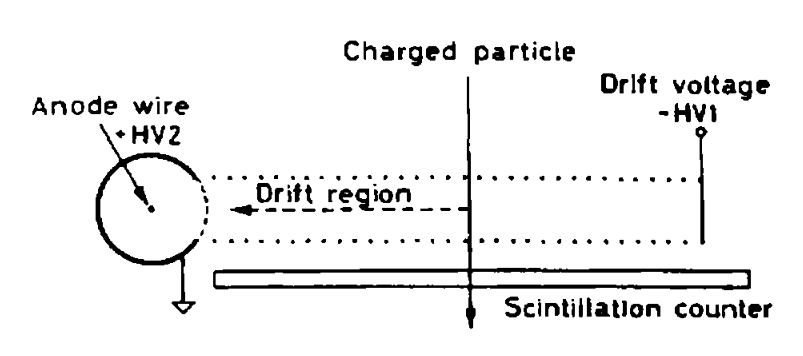
\includegraphics[width=0.6\textwidth]{drift_chamber.png}
	\caption{Schematic of a typical drift chamber. The scintillator counter is placed below the chamber. The 
	traversing charged particle ionizes the gas molecules, and the electrons drift with a constant drift velocity (due to the 
	applied drift voltage) towards the 
	anode, where the signal is created. Obtained from Ref. \cite{Leo1994}.}
	\label{fig:drift_chamber}	
\end{figure*}


The drift chamber is constructed by placing a series of cathode field wires at appropriate voltages in between a high voltage electrode and 
an anode of a simple proportional counter. A scintillation counter is placed before or after the chamber to signal the arrival of a particle. Refer to 
Sec.  \ref{sec:scint_pmt} for more details about the scintillator counter. 
Once the charged particles passes through the chamber and scintillator, the liberated electrons drift to the anode. The fast signal from the scintillator
starts a timer at the same time. The timer is then stopped from the signal created at the anode by the drifting electrons. See Fig. \ref{fig:drift_chamber} for a schematic of a typical 
drift chamber \cite{Leo1994}. In our experiment, we use multiple straws with several layers to more accurately determine the position of the 
atmospheric muons. \par 

\section{Scintillation Detectors and Photomultiplier Tubes} \label{sec:scint_pmt}

Certain materials emit a small flash of light, i.e. a scintillation, when they are struck by nuclear particles or radiation.
With an amplifying device such as a photomultiplier tube (PMT), one can convert the scintillation into an electric pulse
using a scintillation detector. The electric pulse is then analyzed to study about the incident radiation. Scintillation detectors 
are useful especially due to their high sensitivity to energy measurements, their fast time response, and their ability 
to discriminate between pulse shapes. \par 

A scintillator detector is constructed from a scintillating materia which is optically coupled to a PMT. The radiation excites the 
atom or molecule in the scintillating material, causing scintillation to occur. The PMT then converts and amplifies the light into 
an electric current which is then read out by an electronics system \cite{Leo1994}. The scintillation detectors used in our experiment 
operate under the same principles as above. \par 


The photomultiplier tubes used within the scintillation detectors convert detected photons into electronic current that can 
be measured. The photons are collected from a photocathode before emitting an electron due to the photoelectric effect. The electrons 
are then multiplied by a series of dynodes which emits secondary electrons within the material due to transfer of energy. An applied 
voltage is also applied in this region to accelerate these electrons, subsequently producing more electrons. The constructed cascade is 
collected at the anode to give a measurable electronic current \cite{Leo1994}. Fig. \ref{fig:pmt_schematic} shows the schematic of a typical photomultiplier tube. 


\begin{figure*}[!h]
	\centering
	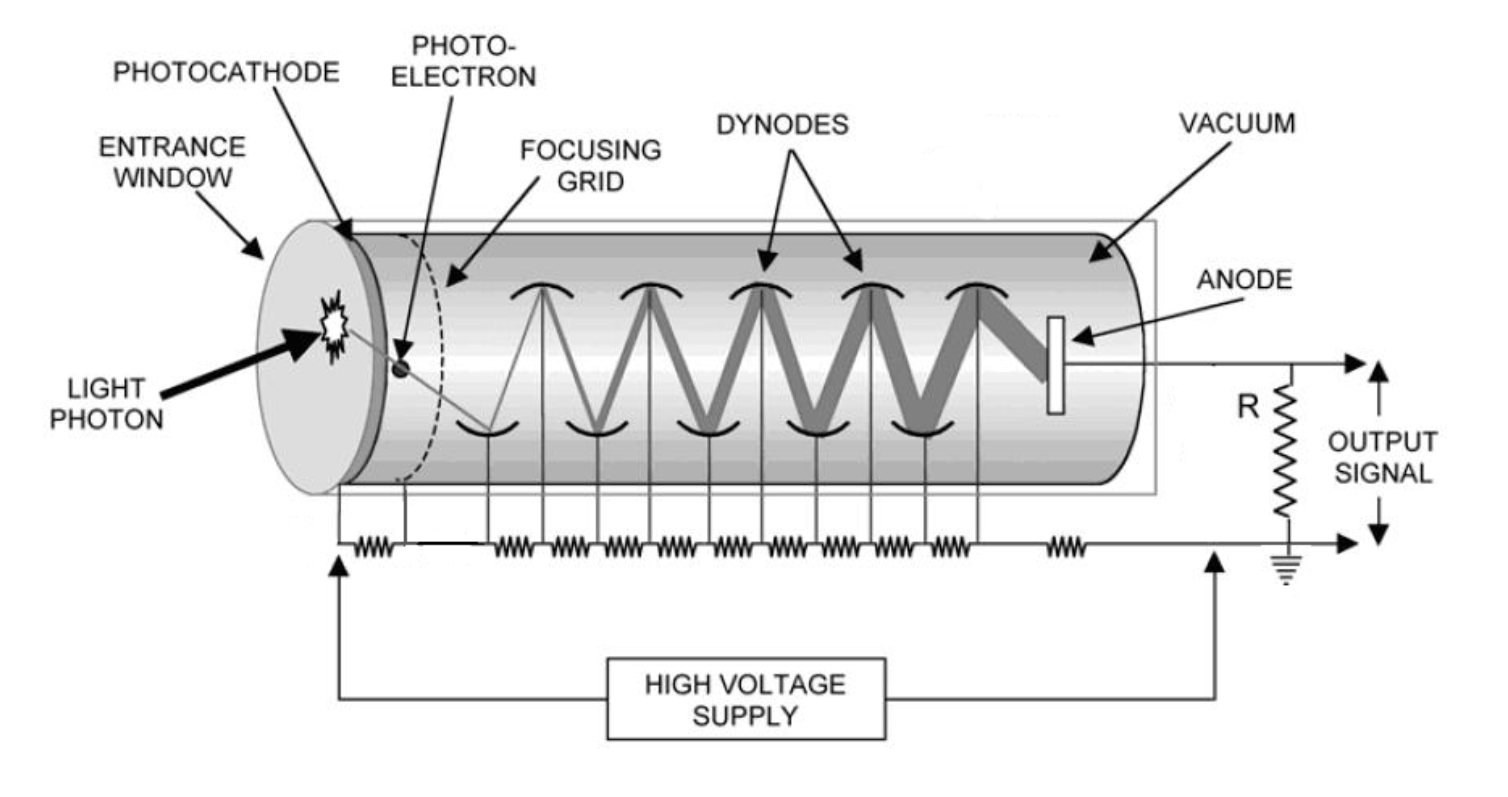
\includegraphics[width=0.6\textwidth]{pmt_schematic.png}
	\caption{Schematic of a typical photomultiplier tube. Photons are detected at the cathode, before entering the focusing grid,
	 and the electrons are accelerated by the multiple dynodes before collected at the anode to produce an electronic signal.
	 Obtained from Ref. \cite{Danisch2014}.}
	\label{fig:pmt_schematic}	
\end{figure*}


\chapter{Experimental Setup} \label{chap:exp_setup}

\section{Detectors}


The experimental setup is shown in fig. \ref{fig:setup1}. The setup consists of two major components, the modules, which are the three copper-colored trapezoids, and the trigger system, which are the two black panels. 

\begin{figure}[htpb]
    \centering
    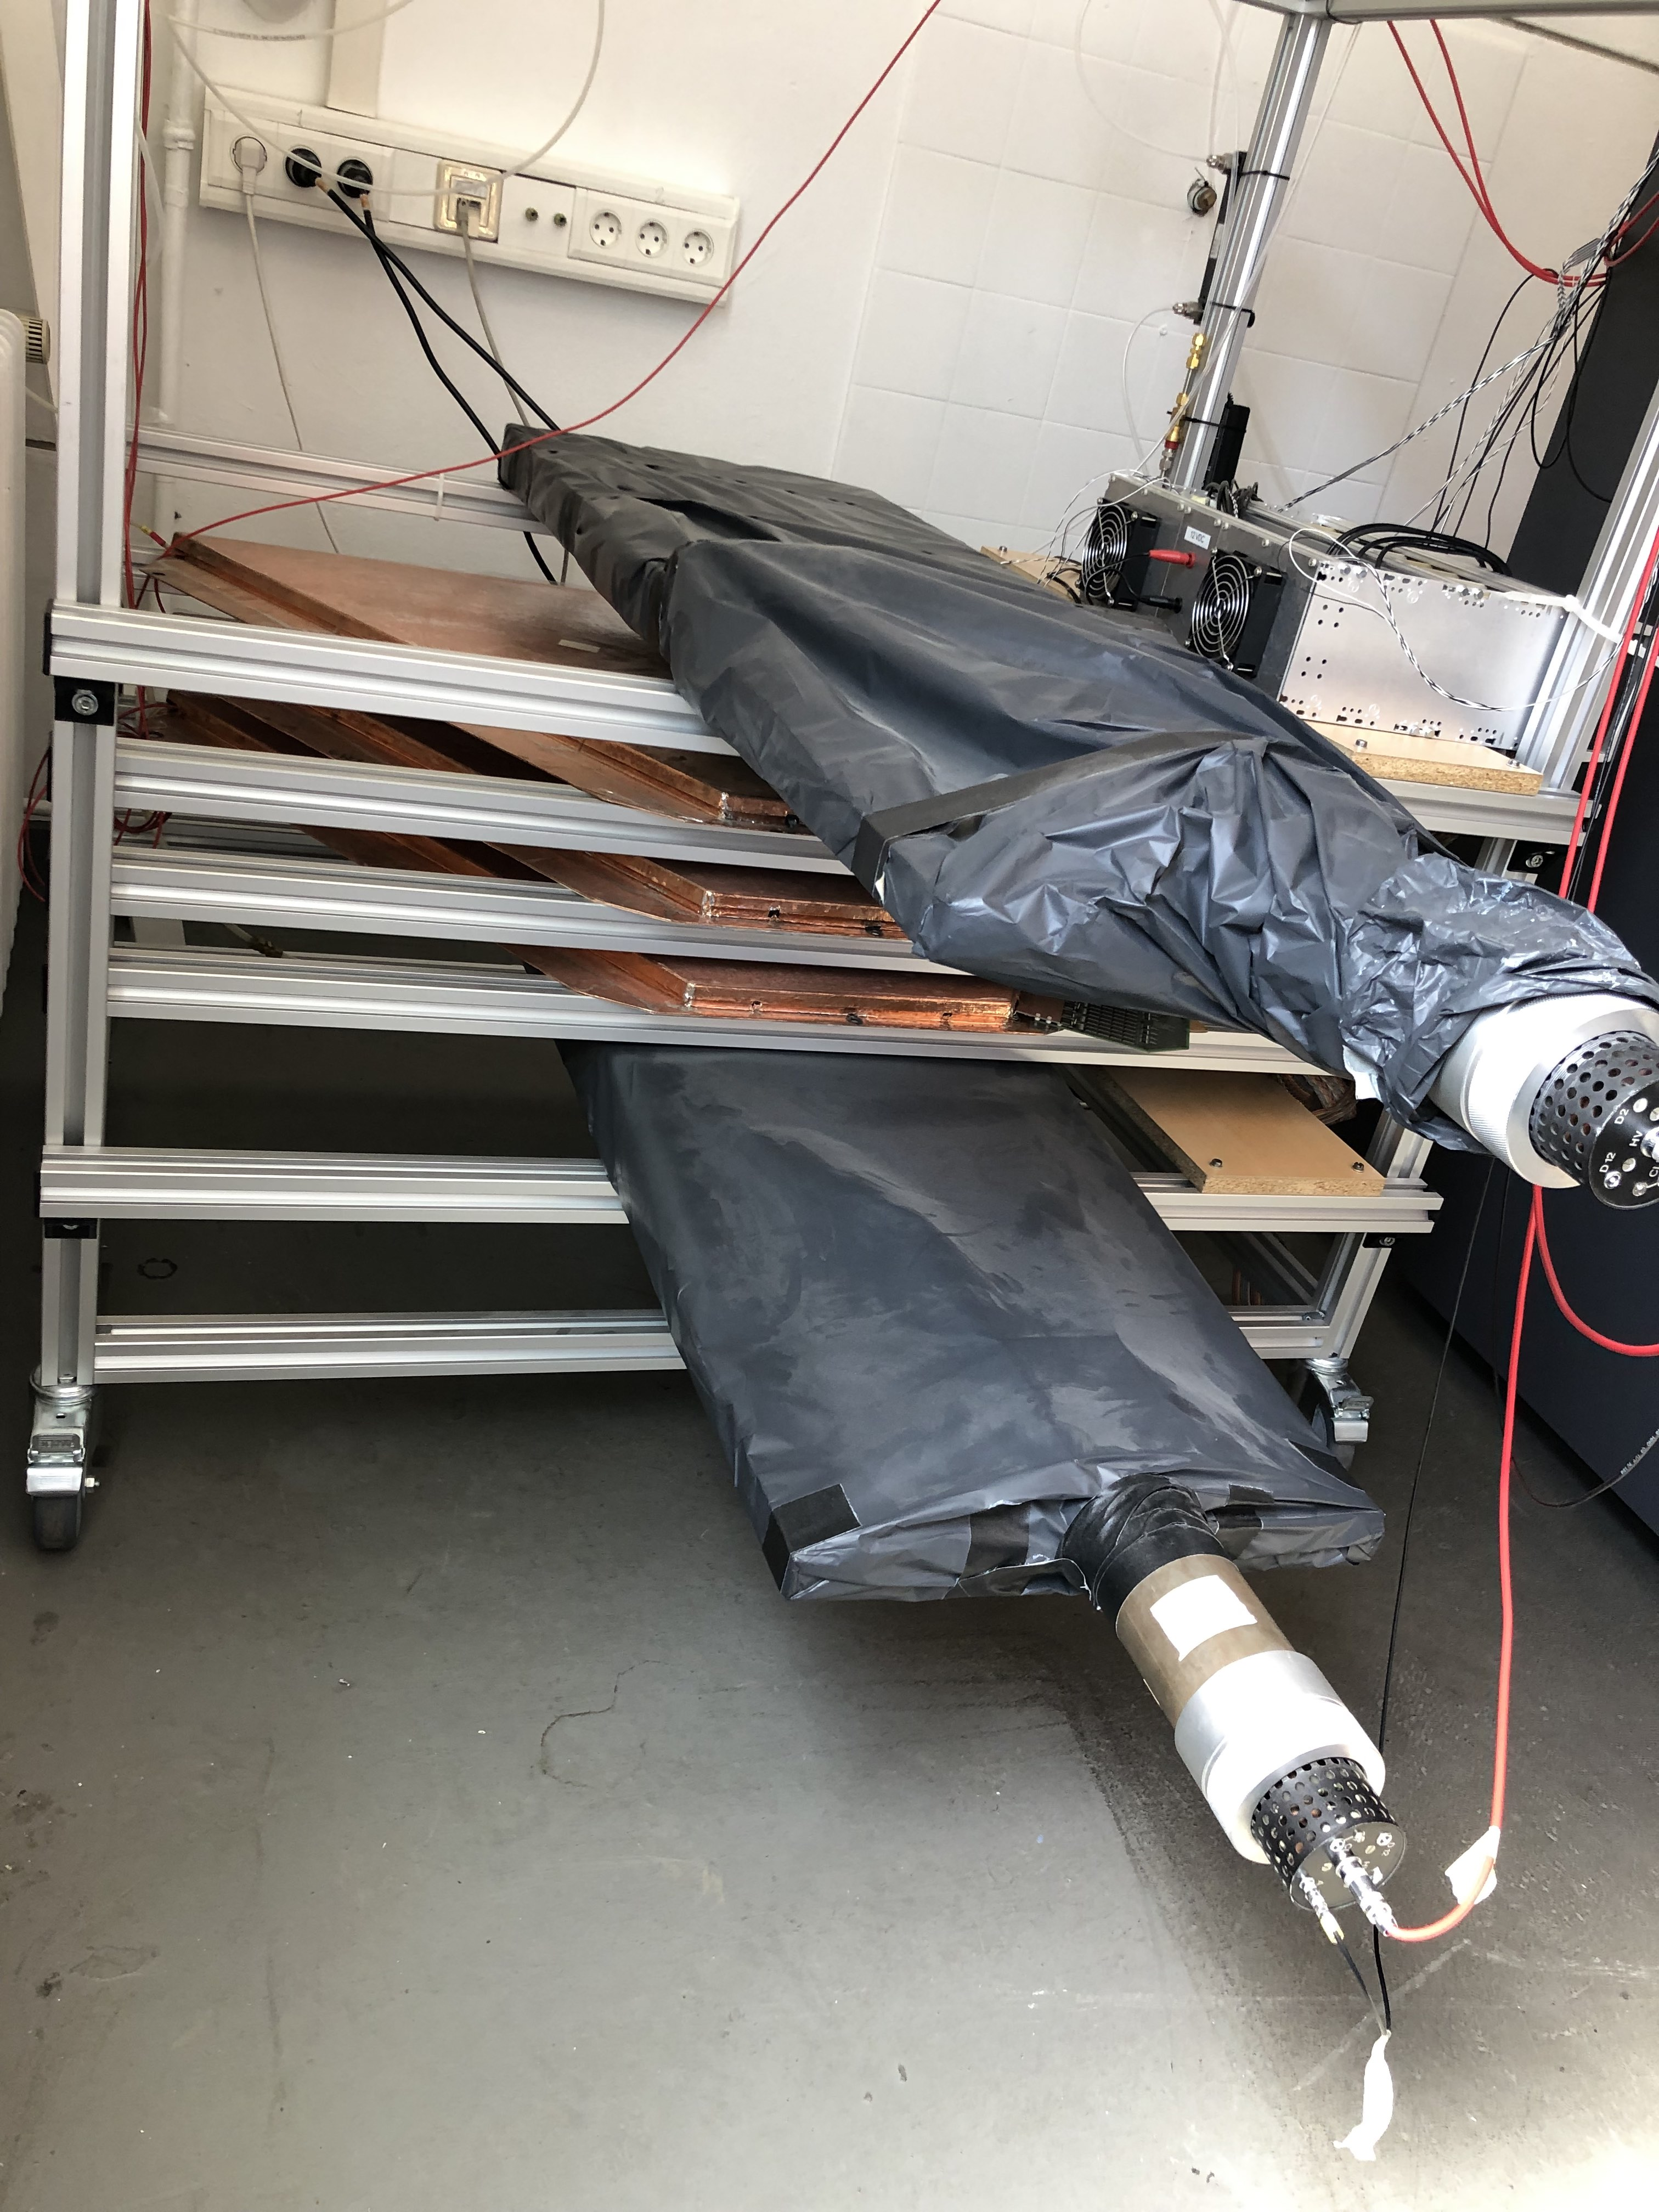
\includegraphics[width=0.6\textwidth]{setup1.jpg}
    \caption{Experimental setup with modules (copper-colored trapezoid) and PMTs (black panels).}
    \label{fig:setup1}
\end{figure}	

The modules consist of simple drift chambers. Each of these modules consists of three layers of 88 straws. The straws are a simple drift chambers, filled with a gas mixture of argon and carbon-dioxide. The radius of each straw is 3.75mm and the length ranges from 20cm to 102cm. The reason for the variable length is due to the trapezoidal shape of the module. Each of these straws is connected to readout channel in a front-end (FE) board which contains a preamplifier, a shaper and a discriminator. When the input voltage exceeds a certain threshold voltage, each of these straws give a digital output pulse. This output pulse is then time-multiplexed for six straws each, which gives an output signal with 200ns offset with respect to each other, giving a total of 1200ns readout window per event. From the FE board, the signal is fed into the TDC board to measure drift time.  

Since the detectors themselves do not have an internal triggering mechanism, an external one is used. This triggering system comprises of two large scintillators which are placed above and below the modules. To these scintillators, photomultiplier tubes (PMTs) are attached which registers the photon emitted by the material when a charged particles passes through and ionizes the material. This light signal is then converted to electronic pulse, which can be measured. Further, the two scintillators are operated in coincidence logic to trigger events when a muon passes both the scintillators and hence the tracking modules. 

\chapter{Procedure}

\section{Determination of PMT Operation Voltage}
Before making the measurements, the operation voltage for the PMT needs to be determined. In order to have a working trigger system, a high voltage needs to be set for the photomultipliers. The voltage is varied in the range of 1700-2300V. The counts measured by the lower photomultiplier are displayed on the middle counter in the electronics rack (as seen in fig. \ref{fig:rack}). In order to reduce the statistical uncertainty, four measurements for each voltage were measured. The result is shown in fig. \ref{fig:low_count}. A change in upper photomultiplier voltage does not affect the count. A standard error of 0.5V is taken for each reading based on the instrumentation. 

\begin{figure}[htpb]
    \centering
    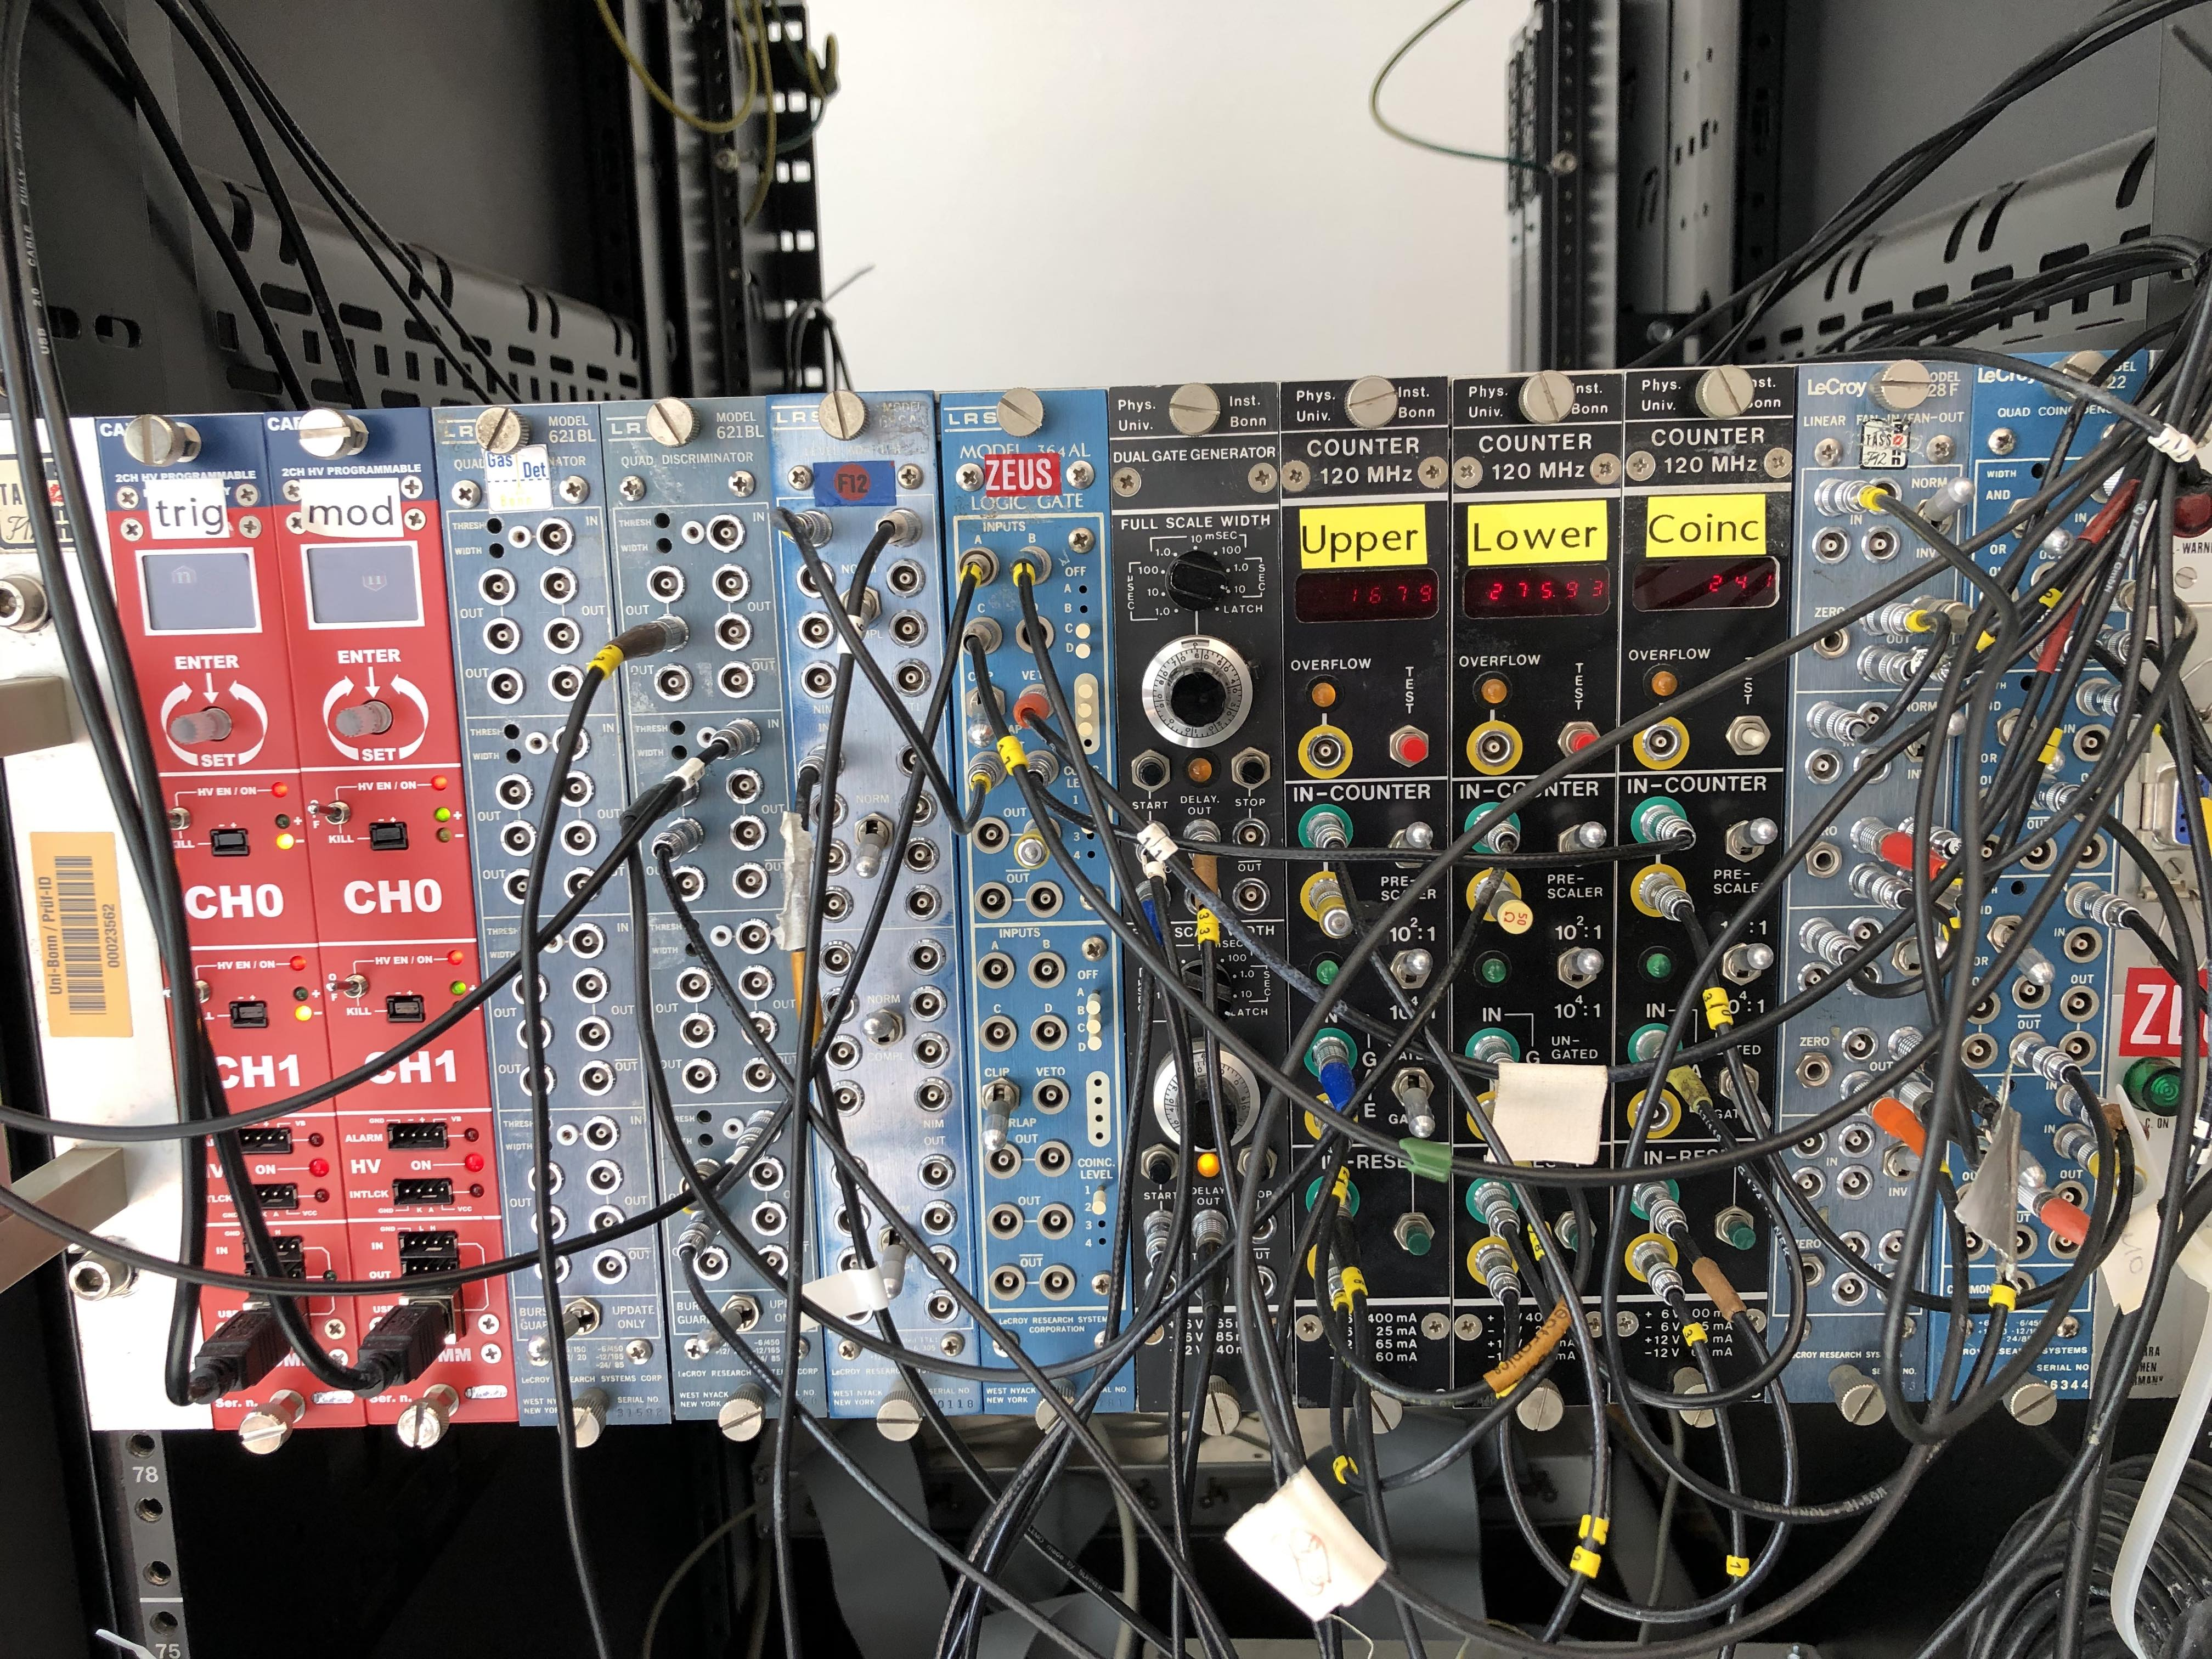
\includegraphics[width=0.6\textwidth]{rack.jpg}
    \caption{The electronic rack which displays the count for upper and lower photomultiplier and the coincidence rate.}
    \label{fig:rack}
\end{figure}	

\begin{figure}[htpb]
    \centering
    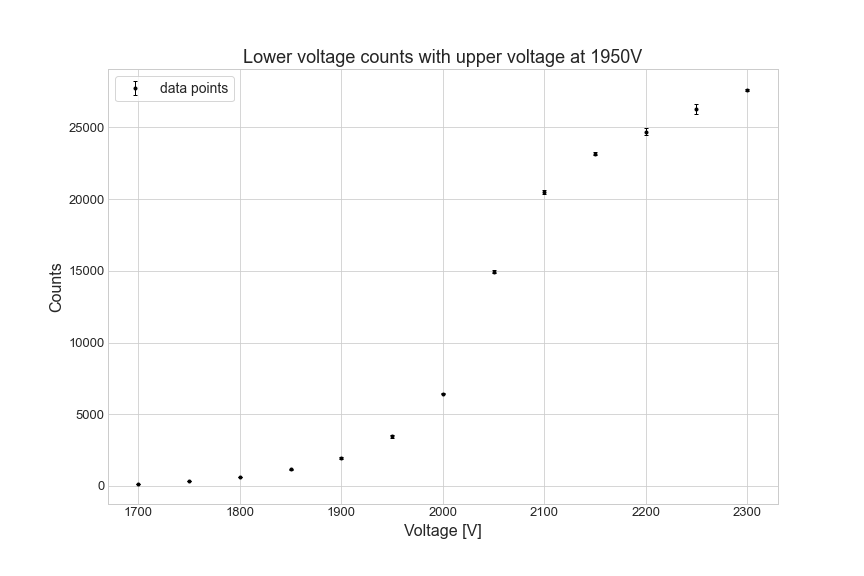
\includegraphics[width=0.8\textwidth]{low_count}
    \caption{The change in count with respect to voltage. We notice an exponential growth followed by a linear growth.}
    \label{fig:low_count}
\end{figure}	

We notice that from 1700-2050V, the behavior is exponential and after 2100V, the behavior is linear. Therefore, we choose the operating voltage for the lower photomultiplier to be 2100V, since above this value, an increase voltage leads to an increase in noise. 

Having fixed the voltage for the bottom panel, we determine the operating voltage for the upper panel. This is done by varying the voltage in the same range but this time instead of measuring the count, we measure the coincidence rate. Again, we take four measurements per voltage to reduce statistical uncertainty. The result is shown in fig. \ref{fig:up_count}. 

\begin{figure}[htpb]
    \centering
    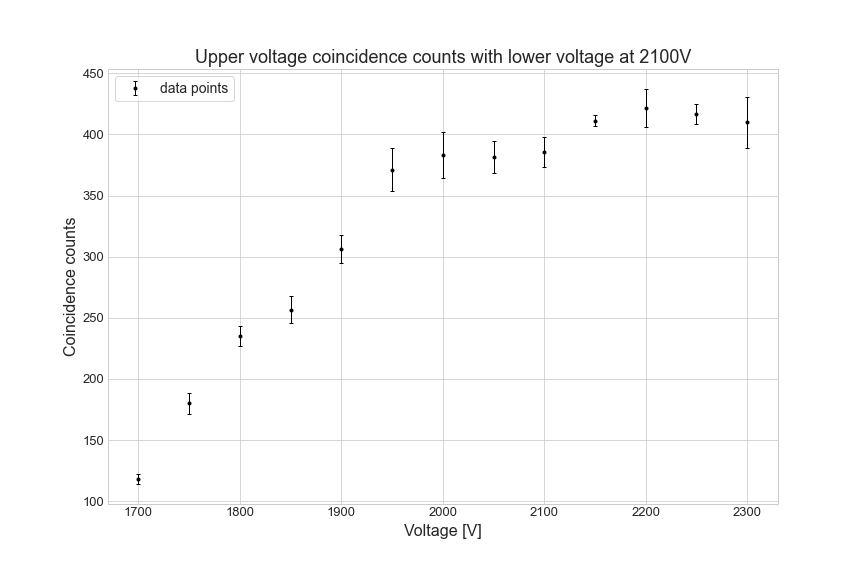
\includegraphics[width=0.8\textwidth]{up_count}
    \caption{The change in coincidence rate with respect to voltage. We notice a plateau, indicating the independence of coincidence rate.}
    \label{fig:up_count}
\end{figure}

A plateau can be seen starting after 1950V. This implies that a subsequent increase in voltage does not change the coincidence rate - the coincidence rate is independent of increase in the voltage. Therefore, we pick 2000V as the operating voltage for the upper panel. 

\section{Front-end Threshold Voltage}

Having determined the optimal operating voltage for the lower and the upper panel, the threshold voltage for front-end has to be determined. To do this, the voltage is varied 1.0-2.6V in the steps of 0.4V. An additional 2.0V reading was also taken. For each voltage, 25000 events are measured. We illustrate the typical procedure below. 

After taking the measurement for 1.0V, the following command is run:

\begin{tcolorbox}
\begin{verbatim}
StyxM2C2 -N 25000 -O TS_10V.txt --all --no-clean \ 
 -I /home/styx/data/etraxp114/te13085163152.hld
\end{verbatim}
\end{tcolorbox}

in order to process the data. The \texttt{StyxM2C2} calls the program. \texttt{-N 25000} considers only the first 25000 events to process them. \texttt{-O TS\_10V.txt} names the output file. \texttt{--all --no-clean} process the data files with \texttt{StyxM2C2} using all process steps except for the cleaning. \texttt{-I \slash home\slash styx\slash data\slash etraxp114\slash te13085163152.hld} is the input file. This is repeated for each voltage. 

To find good channels, the a monitoring root file is produced using the command: 

\begin{tcolorbox}
\begin{verbatim}
StyxMonitor TS_10V_mon.txt
\end{verbatim}
\end{tcolorbox}
This create a \texttt{TS\_10V\_mon.root} file, which can be opened via running:

\begin{tcolorbox}
\begin{verbatim}
root TS_10V_mon.root
\end{verbatim}
\end{tcolorbox}
After \texttt{root} has started, the command \texttt{new TBrowser} is used to browse through the plots and study them. To compare the results from one TDC number and one channel number, the following command is run: 

\begin{tcolorbox}
\begin{verbatim}
StyxThresholdScan 1 3 TS_10V_mon.txt TS_14V_mon.txt TS_18V_mon.txt TS_20V_mon.txt\ 
TS_22V_mon.txt TS_26V_mon.txt
\end{verbatim}
\end{tcolorbox}
This would then compare the channel 3 and TDC 1 for all the measurements. 


\section{Overnight Measurement}

\printbibliography

\end{document}
